\documentclass[11pt]{article}

\usepackage[T1]{fontenc}
\usepackage{mathtools,amsthm,amssymb}
\usepackage{lmodern}
\usepackage{microtype}
\usepackage[margin=1.05in]{geometry}
\usepackage{enumitem}
\usepackage{needspace}
\usepackage{xcolor}
\usepackage{tikz}
\usetikzlibrary{arrows.meta}
\pdftrailerid{}
\pdfsuppressptexinfo=15
\usepackage{hyperref}
\hypersetup{colorlinks=true,linkcolor=black,citecolor=black,
  urlcolor=blue!45!black,pdftitle={The second Kahn--Kalai conjecture}}

\newtheorem{theorem}{Theorem}[section]
\newtheorem{lemma}[theorem]{Lemma}
\numberwithin{equation}{section}

\newcommand{\PP}{\mathbb P}
\newcommand{\EE}{\mathbb E}
\newcommand{\pc}{p_{\mathrm c}}
\newcommand{\pE}{p_{\mathrm E}}
\newcommand{\ind}{\mathbf 1}
\newcommand{\TT}{\mathcal T}
\newcommand{\UU}{\mathcal U}
\newcommand{\ch}{\operatorname{Ch}}
\newcommand{\ee}{\mathrm e}
\newcommand{\src}{\mathsf c}
\newcommand{\tgt}{\mathsf b}
\newcommand{\GG}{\boldsymbol\Gamma}
\newcommand{\qs}{q_*}
\newcommand{\step}[2]{\par\medskip\noindent\textbf{Step #1 (#2).}\ }
\newcommand{\unverified}[1]{\par\smallskip\noindent\fbox{\parbox{0.95\linewidth}{\textbf{Unverified step.} #1}}\par\smallskip}

\title{The second Kahn--Kalai conjecture}
\author{Rewritten for readability from the OpenAI manuscript of the same title}
\date{}

\begin{document}
\maketitle
\begin{abstract}
We prove the second Kahn--Kalai conjecture. For every finite simple graph
$H$ with $h\ge1$ edges and at most $n$ vertices, the threshold for
$G(n,p)$ to contain an ordinary copy of $H$ is at most
$C p_{\mathrm E}(n,H)(1+\log_2 h)$, where $C$ is universal.
Here $p_{\mathrm E}(n,H)$ is the least density at which every subgraph
of $H$ has expected copy count at least one half.
\end{abstract}

\section{The main result and how it is proved}\label{sec:introduction}

\subsection{Definitions and statement}

All graphs are finite and simple; $v(F)$ and $e(F)$ are the numbers of
vertices and edges of $F$. A \emph{subgraph} of $G$ is a graph whose
vertex set and edge set are subsets of those of $G$. A \emph{copy} of $F$
in $G$ is a subgraph of $G$ isomorphic to $F$, and $N(G,F)$ is the number
of copies. These are ordinary copies: $G$ may have additional edges
between the vertices of a copy. Let $K_n$ be the complete graph on
$[n]=\{1,\ldots,n\}$ and let $G(n,p)$ be the random graph on $[n]$ in
which each edge of $K_n$ is present independently with probability $p$.
Each copy of $F$ in $K_n$ has $e(F)$ edges and so lies in $G(n,p)$ with
probability $p^{e(F)}$; by linearity of expectation,
\begin{equation}\label{eq:expect}
 \EE N(G(n,p),F)=N(K_n,F)\,p^{e(F)}.
\end{equation}
For a graph $H$ with at least one edge and at most $n$ vertices, define
\begin{align*}
 \pc(n,H)
 &=\inf\{p\in[0,1]:\PP(N(G(n,p),H)>0)\ge\tfrac12\},\\
 \pE(n,H)
 &=\inf\{p\in[0,1]:\EE N(G(n,p),F)\ge\tfrac12
                 \text{ for every subgraph }F\subseteq H\}.
\end{align*}
The first is the \emph{containment threshold}, the second the
\emph{graph expectation threshold}. Three elementary facts:
\begin{enumerate}[label=(\alph*),leftmargin=2.2em,itemsep=2pt]
 \item \emph{Both infima are attained.} The probability and the
 expectations are polynomials in $p$, hence continuous, so each set of
 admissible $p$ is closed; there are finitely many constraints; and
 $p=1$ satisfies all of them, because $K_n$ contains a copy of $H$ (as
 $v(H)\le n$) and hence of every $F\subseteq H$.
 \item \emph{$\pE(n,H)>0$.} A single edge is a subgraph of $H$, and by
 \eqref{eq:expect} its constraint is $\binom n2p\ge\frac12$.
 \item \emph{$\pE(n,H)\le\pc(n,H)$.} By (a) the defining inequality of
 $\pc$ holds at $p=\pc(n,H)$ itself: there $G(n,p)$ contains $H$, hence
 every $F\subseteq H$, with probability at least $\frac12$, so
 $\EE N(G(n,p),F)\ge\PP(N(G(n,p),F)\ge1)\ge\frac12$.
\end{enumerate}

\begin{theorem}\label{thm:main}
For every $n\ge2$ and every finite simple graph $H$ with $h=e(H)\ge1$
edges and at most $n$ vertices,
\begin{equation}\label{eq:stronger}
 \pc(n,H)\le
 \min\{1,\;2048\ee^{50}\pE(n,H)(1+\log_2 h)\}.
\end{equation}
In particular,
\[
 \pc(n,H)\le6144\ee^{50}\pE(n,H)\log_2 n.
\]
\end{theorem}

Here $\ee$ is the base of the natural logarithm (not to be confused with
the edge count $e(\cdot)$). The constants are explicit and universal;
$H$ may vary with $n$.

\emph{Normalization.} Kahn and Kalai use expected count one instead of
one half. Write $\pE^{(1)}(n,H)$ for the threshold defined with $1$ in
place of $\frac12$ (this symbol is used only in this remark). Then
$\pE\le\pE^{(1)}\le2\pE$. Indeed, by \eqref{eq:expect}, for a subgraph
$F$ with $e\ge1$ edges the constraint $\EE N(G(n,p),F)\ge\theta$ reads
$p\ge(\theta/N(K_n,F))^{1/e}$, and passing from $\theta=\frac12$ to
$\theta=1$ multiplies this lower bound by $2^{1/e}\in(1,2]$; a subgraph
without edges has constant expected count $N(K_n,F)\ge1$ and constrains
$p$ in neither case. Each threshold is the largest of these lower
bounds. Since $\pc$ does not involve the normalization, the two
versions of the conjecture differ only in the value of the universal
constant.

\paragraph{Conventions.}
$\log$ is the natural logarithm. For a finite set $X$ and
$0\le\rho\le1$, $\mu_\rho$ is the law of a random subset of $X$ that
contains each element independently with probability $\rho$; we also
write $\mu_\rho(y)=\rho^{|y|}(1-\rho)^{|X|-|y|}$ for the probability of
a set $y\subseteq X$. A graph on $[n]$ is determined by its edge set, a
subset of $X=\binom{[n]}2$, and the edge set of $G(n,p)$ has law $\mu_p$.

\subsection{Proof at a glance}\label{sec:glance}

\paragraph{What has to be shown.}
Let $r$ be the right-hand side of \eqref{eq:stronger}. By the definition
of $\pc$ it suffices to show that a $\mu_r$-random subset of
$X=\binom{[n]}2$ contains the edge set of a copy of $H$ with probability
at least $\frac12$. The proof gives $\frac23$.

\paragraph{Key idea.}
A copy of $H$ is built in stages
$\varnothing=H_0\subset H_1\subset\cdots\subset H_k$ (edge sets, $H_k$
being all of $H$), each stage adding more than $16$ times as many edges
as the previous one. The stages are chosen so that, given any copy of
$H_{i-1}$, a uniformly random extension to a copy of $H_i$ adds an edge
set whose law is \emph{$\sigma$-spread} with $\sigma=128\,\pE(n,H)$:
every fixed set $J$ of edges is contained in the added set with
probability at most $\sigma^{|J|}$. All stage-by-stage constructions are
stored in one rooted tree whose arcs are labelled by the added edge
sets. A random set $W$ of density $\rho=4\ee^{50}\sigma$ is then used
to shrink \emph{all} arcs of the tree at once: each label is replaced by
its part outside $W$, and enough of the tree survives that the size
bound at every level is halved, while the spread constant barely
changes. After $\lfloor\log_2 h\rfloor+1$ such rounds nothing is left
to cover, so the union of the sets $W$ that were used contains a copy of
$H$. Using the same $W$ at all levels creates dependence between
levels. The mechanism that controls it is this: the labels along any
root-to-leaf path of the tree are pairwise disjoint (successive stages
add disjoint edge sets), so everything computed in the subtree below an
arc depends on $W$ only outside that arc's label
(Lemma~\ref{lem:reduction}, Step~4), and for such quantities
Lemma~\ref{lem:local} gives a change-of-measure bound
(Lemma~\ref{lem:reduction}, Step~5).

\paragraph{The steps and their dependencies.}
\begin{enumerate}[leftmargin=2em,itemsep=2pt]
 \item \textbf{Lemma~\ref{lem:local} (one family).} For a single
 $a$-spread family of sets of size at most $m$ and $W\sim\mu_\rho$ with
 $a/\rho\le\ee^{-50}$, a random ``transition'' replaces a set $A$ of the
 family by a fragment $T=A\setminus W$. The lemma gives (i) $|T|\le m/2$
 except with probability $\ee^{-9m}$, and (ii) a change-of-measure bound
 with cost $\ee^{11m}$ for functions of $W$ outside $A$.
 \item \textbf{Lemma~\ref{lem:reduction} (one round on a tree).}
 Applies step 1 at every node with one common $W$. Part (ii) of step 1
 together with disjointness along paths shows that, with probability at
 least $\frac34$, a subtree survives in which all capacities are halved.
 \item \textbf{Theorem~\ref{thm:tree} (tree covering).} Iterates
 step 2. This is where the factor $1+\log_2\ell_k$ arises: it is the
 number of halvings.
 \item \textbf{Lemma~\ref{lem:hierarchy} (graph hierarchy).} Builds the
 tree for $H$. This is the only place where graphs and $\pE$ enter.
 \item \textbf{Theorem~\ref{thm:main}} is Theorem~\ref{thm:tree}
 applied to the tree of Lemma~\ref{lem:hierarchy}.
\end{enumerate}
\[
 \text{Lemma~\ref{lem:local}}\Longrightarrow
 \text{Lemma~\ref{lem:reduction}}\Longrightarrow
 \text{Theorem~\ref{thm:tree}}\Longrightarrow
 \text{Theorem~\ref{thm:main}}\Longleftarrow
 \text{Lemma~\ref{lem:hierarchy}}.
\]
Sections~\ref{sec:resampling} and~\ref{sec:trees} concern set systems
only and can be read without Section~\ref{sec:graphs}.

\paragraph{Where the constant comes from.}
$2048=128\cdot4\cdot4$: the hierarchy has spread $\sigma=128\,\pE$; over
all rounds the spread constant grows by a factor less than $4$; and
$4s$ rounds are allowed for $s=\lfloor\log_2\ell_k\rfloor+1$ successes.
The factor $\ee^{50}$ is the ratio $\rho/a$ required by
Lemma~\ref{lem:local}.

\paragraph{Notation changes relative to the source.}
Only names are changed, to give each symbol one meaning. The random
source and target of the transition are written $\src,\tgt$, and
$c,b$ denote their values. The summation index in $Z$ is $b'$. In
Lemma~\ref{lem:reduction} the outgoing level of the current node is
always $j$ (the source also used $s$), and summation indices are $i,g$
(the source used $j,h$). In the proof of Theorem~\ref{thm:tree} the
number of successes so far is $\tau$ (source: $t$). In
Section~\ref{sec:graphs} the number $\pE(n,H)$ is written $\qs$
(source: $q$), to keep it apart from the functionals $q(\cdot)$,
$q_f(\cdot)$ of Section~1.3; a uniform random copy of $I$ is $\GG_I$
(source: $\boldsymbol I$), $|S|$ is $\kappa$ (source: $r$), and the edge
set of $H$ is written $E(H)$ rather than $H$.

\subsection{Context and attribution (not used in the proofs)}

Nothing in this subsection is used in
Sections~\ref{sec:resampling}--\ref{sec:graphs}. The statements quoted
here are results of the cited works; they are reported, not proved or
rechecked, here.

\paragraph{The conjecture.}
By fact (c), a necessary condition for containing $H$ is that every
subgraph of $H$ have a reasonable expected number of copies. Kahn and
Kalai~\cite{KK07} conjectured that this obstruction determines the
containment threshold within a logarithmic factor, uniformly over the
target graph. Theorem~\ref{thm:main} proves this, with the logarithm
depending on the number of target edges. For a fixed target, threshold
questions belong to the classical theory of Erd\H{o}s and
R\'enyi~\cite{ER60}; Bollob\'as~\cite{Bollobas81} treated general fixed
subgraphs. A logarithm is needed when the target grows: for $H$ a
perfect matching on an even number $n$ of vertices,
$\pE(n,H)=\Theta(1/n)$ whereas
$\pc(n,H)=\Theta(\log n/n)$~\cite{ER66,KK07}, the larger scale being
needed to eliminate isolated vertices of the host. Hamilton cycles
exhibit the same gap~\cite{KK07}. Other spanning targets have required
different methods: Riordan~\cite{Riordan00}, for example, proved that
for every fixed $p>1/4$, $G(2^d,p)$ contains the $d$-dimensional cube
with probability tending to one.

\paragraph{The abstract conjecture, and why it does not suffice.}
Let $\mathcal F\subseteq2^X$ be a nonempty proper increasing family on
a finite set $X$. A \emph{cover} is a family $\mathcal G\subseteq2^X$
such that every $F\in\mathcal F$ contains some $S\in\mathcal G$; its
cost at density $p$ is $\sum_{S\in\mathcal G}p^{|S|}$. The integral
expectation threshold $q(\mathcal F)$ is the largest $p$ for which some
cover has cost at most $\frac12$. A fractional cover assigns weights
$w_S\ge0$ with $\sum_{S\subseteq F}w_S\ge1$ for each $F\in\mathcal F$,
has cost $\sum_Sw_Sp^{|S|}$, and defines $q_f(\mathcal F)$ with the
same budget. Union bounds and expectations give
$q(\mathcal F)\le q_f(\mathcal F)\le p_{\mathrm c}(\mathcal F)$, where
$p_{\mathrm c}(\mathcal F)$ is the density at which a $\mu_p$-random
subset belongs to $\mathcal F$ with probability $\frac12$.
Talagrand~\cite[Section~6]{Tal10} introduced the fractional formulation
and its dual description by spread probability measures. Alweiss,
Lovett, Wu, and Zhang~\cite{ALWZ21}, building on the regularity
viewpoint of Lovett, Solomon, and Zhang~\cite{LSZ19}, developed the
fragment method in their work on sunflowers. Frankston, Kahn,
Narayanan, and Park~\cite{FKNP21} proved
$p_{\mathrm c}(\mathcal F)=O(q_f(\mathcal F)\log\ell)$, where $\ell$ is
the maximum of two and the largest size of a minimal member of
$\mathcal F$ (this $\ell$ is unrelated to the capacities $\ell_i$ of
Section~\ref{sec:trees}). Park and Pham~\cite{PP24} proved the
corresponding bound with $q$ in place of $q_f$, resolving the abstract
Kahn--Kalai conjecture by a minimum-fragment argument. The integral and
fractional thresholds are within a universal constant factor at the
common one-half
budget~\cite[Theorem~1.1]{OpenAIThresholdEquivalence2026}. This
comparison is contextual; the proof below does not use it.

Let $\mathcal F_H$ be the family of edge sets on $[n]$ containing a copy
of $H$. Then $\pE(n,H)\le q(\mathcal F_H)$, for the following reason.
Take any $p<\pE(n,H)$ (possible by fact (b)). By the definition of
$\pE$ some subgraph $F\subseteq H$, depending on $p$, has
$\EE N(G(n,p),F)<\frac12$. Every member of $\mathcal F_H$ contains a copy
of $H$, hence the edge set of a copy of $F$. So the edge sets of the
copies of $F$ in $K_n$ form a cover, and by \eqref{eq:expect} its cost
at $p$ is at most $\EE N(G(n,p),F)<\frac12$. Hence
$q(\mathcal F_H)\ge p$ for every $p<\pE(n,H)$. The inequality goes the
wrong way for our purpose: the abstract theorem bounds $\pc$ by
$O(q(\mathcal F_H)\log)$, which does not bound it in terms of the
possibly smaller $\pE(n,H)$.

\paragraph{Earlier graph results.}
Mossel, Niles-Weed, Sun, and Zadik~\cite[Theorem~1]{MNSZ22} obtained a
single logarithm using the modified graph threshold
\[
 \widetilde p_{\mathrm E}(n,H)
 =\min\{p:\EE N(G(n,p),F)\ge N(H,F)/2
                  \text{ for every }F\subseteq H\},
\]
where the factor $N(H,F)$ records that containing $H$ supplies all its
copies of $F$. By symmetry this parameter equals
$q_f(\mathcal F_H)$~\cite[Equation~(1)]{DKP25}; this identity is quoted
from that reference and is not proved or used here. Comparing it with
$\pE(n,H)$ is the additional graph-specific problem. Dubroff, Kahn, and
Park~\cite[Theorems~1.2--1.5]{DKP25} proved
$q_f(\mathcal F_H)=O(\pE(n,H)\log^2 n)$ and hence
$\pc(n,H)=O(\pE(n,H)\log^3 n)$, using a rooted-extension decomposition,
and established the single-logarithm bound when $\pE(n,H)<1/(3n)$. In
further work~\cite[Theorems~1.4--1.5]{DKP25Cases} they proved
$N(H,F)\le\EE N(G(n,\min\{1,Lq\}),F)$ whenever all subgraphs of $H$ have
expected count at least one at a density $q$, for test graphs $F$ that
are cliques, cycles, or bounded-degree trees ($L$ universal for cliques
and cycles, depending on the degree bound for trees).
Tran~\cite{Tran26} then obtained
$q_f(\mathcal F_H)=O(\pE(n,H)\log(2e(H)))$, reducing the general
containment loss to $O(\log^2(2e(H)))$, and removed the loss in the
comparison of expectation thresholds for trees and for graphs whose
average degree is at least the logarithm of their maximum degree,
thereby proving the second conjecture for these classes.

\paragraph{What is taken from earlier work and what is new.}
In the account above, the route through $q_f(\mathcal F_H)$ pays two
logarithms: one in bounding $q_f(\mathcal F_H)$ by $\pE$, and one in
passing from $q_f$ to $\pc$ via~\cite{FKNP21}. The present proof never
forms $q_f(\mathcal F_H)$, that is, it never needs one spread measure on
whole copies of $H$. From Tran~\cite[Section~3, Lemma~3.1]{Tran26} it
takes the ratio-maximizing choice of a subgraph $S\subseteq I$ and the
resulting spread of each \emph{conditional} extension law; this costs
the constant $128$ and no logarithm (Lemma~\ref{lem:hierarchy}, proved
in full below). The conditioning step has antecedents in the large-link
argument of Lovett, Solomon, and Zhang~\cite[Claim~29]{LSZ19} and the
spread-link extraction from a maximal violating core in Alweiss, Lovett,
Wu, and Zhang~\cite[Lemma~2.4]{ALWZ21}. The copy-count identity
\eqref{eq:copy-ratio} also appears in~\cite[Equation~(5)]{MNSZ22}. The
transition of Section~\ref{sec:resampling} is the planted-set and
posterior-resampling construction of Mossel, Niles-Weed, Sun, and
Zadik~\cite[Sections~2.1--2.3]{MNSZ25}; Lemma~\ref{lem:local} adds a
capacity-dependent failure estimate and a change-of-measure bound.
Tran~\cite[Section~4]{Tran26} proposed a coupling conjecture that would
absorb successive conditional extensions while paying the logarithmic
sampling cost once. Theorem~\ref{thm:tree} proves the required
containment bound instead by a tree reduction: all possible extension
histories are kept in a tree, every level is reduced with the same
random set, and the logarithm is paid once.

\section{Resampling one spread family}\label{sec:resampling}

This section concerns a single weighted family of sets. Its result,
Lemma~\ref{lem:local}, is applied in Section~\ref{sec:trees} at every
node of a tree.

\paragraph{Weighted families and spread.}
Throughout this section $X$ is a finite set and $0<\rho<1$. A
\emph{weighted family} on $X$ consists of a finite index set $B$, a
\emph{label} $A_b\subseteq X$ for each $b\in B$, and weights $\nu_b>0$
with $\sum_{b\in B}\nu_b=1$. Distinct indices may have the same label,
and labels may be empty. For $a>0$ the family is \emph{$a$-spread} if
\begin{equation}\label{eq:spread}
 \PP_{c\sim\nu}(J\subseteq A_c)
 =\sum_{b\in B:\,J\subseteq A_b}\nu_b\le a^{|J|}
 \qquad(\varnothing\ne J\subseteq X).
\end{equation}

\paragraph{The transition.}
For $y\subseteq X$ put
\begin{equation}\label{eq:Z}
 Z(y)=\sum_{b'\in B}\nu_{b'}\rho^{-|A_{b'}|}
                  \ind_{\{A_{b'}\subseteq y\}}.
\end{equation}
Given a set $W\subseteq X$, the \emph{transition at $W$} produces a
random pair $(\src,\tgt)\in B\times B$ as follows.
\begin{enumerate}[label=\arabic*.,leftmargin=2em,itemsep=2pt]
 \item Choose a \emph{source} $\src$ with law $\nu$, and set
 $Y=W\cup A_{\src}$.
 \item Given $\src=c$, choose a \emph{target} $\tgt$ with
 \begin{equation}\label{eq:posterior}
  \PP(\tgt=b\mid\src=c)=\pi_W(b\mid c):=
  \frac{\nu_b\rho^{-|A_b|}\ind_{\{A_b\subseteq W\cup A_c\}}}
       {Z(W\cup A_c)}.
 \end{equation}
 \item Retain the \emph{fragment} $T=A_{\tgt}\setminus W$.
\end{enumerate}
This is well defined: $Z(W\cup A_c)\ge\nu_c\rho^{-|A_c|}>0$, and
$\sum_b\pi_W(b\mid c)=1$ by \eqref{eq:Z}. So at a fixed $W$ the joint
law is
\begin{equation}\label{eq:joint}
 \PP(\src=c,\ \tgt=b\mid W)=\nu_c\,\pi_W(b\mid c).
\end{equation}

\paragraph{Two regimes.}
``At fixed $W$'' means that $W$ is a given set and probabilities are
over $(\src,\tgt)$ with law \eqref{eq:joint}. ``With $W\sim\mu_\rho$''
means that $W$ is drawn first and then $(\src,\tgt)$ is drawn by
\eqref{eq:joint}, so the triple $(W,\src,\tgt)$ has law
$\mu_\rho(W)\nu_c\pi_W(b\mid c)$. In both regimes the source has law
$\nu$, and in the second it is independent of $W$, since the
$c$-marginal of \eqref{eq:joint} is $\nu_c$ for every $W$. The target
is different: at fixed $W$ its law is $\sum_c\nu_c\pi_W(b\mid c)$,
which in general is not $\nu_b$.

\paragraph{Four properties of the transition.}
\begin{enumerate}[label=(P\arabic*),leftmargin=2.6em,itemsep=3pt]
 \item \emph{The fragment lies in the source label:}
 $T\subseteq A_{\src}\cap A_{\tgt}$. Indeed $\pi_W(b\mid c)>0$ forces
 $A_b\subseteq W\cup A_c$, so $A_b\setminus W\subseteq A_c$. This is
 used to transfer spread from the source to the fragment.
 \item \emph{$W$ and the fragment cover the target label:}
 $A_{\tgt}\subseteq W\cup T$, by the definition of $T$. This does not
 determine $A_\tgt$ from $W$ and $T$; only the covering is used.
 \item \emph{Locality:} the law \eqref{eq:joint}, the value
 $Z(W\cup A_c)$ for each $c$, and the set $A_b\setminus W$ for each $b$
 depend on $W$ only through $W\cap\bigcup_{b'\in B}A_{b'}$. Indeed
 $\ind_{\{A_{b'}\subseteq W\cup A_c\}}
 =\ind_{\{A_{b'}\setminus A_c\subseteq W\}}$, and these indicators
 determine $Z$ and $\pi_W$.
 \item \emph{Law of the planted set:} if $W\sim\mu_\rho$, then
 $\PP(Y=y)=\mu_\rho(y)Z(y)$ for every $y\subseteq X$.
\end{enumerate}

\begin{proof}[Proof of (P4)]
Fix $c$. We have $W\cup A_c=y$ if and only if $A_c\subseteq y$, every
element of $y\setminus A_c$ lies in $W$, and no element of
$X\setminus y$ lies in $W$; elements of $A_c$ are unconstrained. For
$A_c\subseteq y$ this has probability
$\rho^{|y|-|A_c|}(1-\rho)^{|X|-|y|}=\mu_\rho(y)\rho^{-|A_c|}$. Since
$\src$ is independent of $W$, averaging over $c$ with weights $\nu_c$
gives $\mu_\rho(y)Z(y)$. (Sanity check: summing over $y$ gives
$\EE_{\mu_\rho}Z=\sum_b\nu_b\rho^{-|A_b|}\rho^{|A_b|}=1$.)
\end{proof}

\paragraph{Why \eqref{eq:posterior} is called a posterior (not needed
later).}
By the proof of (P4), when $W\sim\mu_\rho$ the conditional law of the
source given $Y=y$ is
$\nu_c\rho^{-|A_c|}\ind_{\{A_c\subseteq y\}}/Z(y)$, which is
\eqref{eq:posterior}. So the target is a second sample from the
conditional law of the source given $Y$.

\begin{lemma}[Local resampling]\label{lem:local}
Let $(A_b)_{b\in B}$ with weights $\nu$ be a weighted family on $X$ and
$m$ a positive integer. Suppose that $|A_b|\le m$ for all $b$, that the
family is $a$-spread, and that
\[
 0<\rho<1,\qquad a/\rho\le\ee^{-50}.
\]
Let $W\sim\mu_\rho$ and perform the transition at $W$. Call the outcome
a \emph{local failure} if
\[
 Z(Y)<\ee^{-10m}\quad\text{or}\quad |T|>m/2.
\]
Then
\begin{equation}\label{eq:local-failure}
 \PP(\text{local failure})\le\ee^{-9m}.
\end{equation}
Moreover, for each fixed $b\in B$ and every nonnegative function $f$ of
subsets of $X$ such that $f(W)$ depends only on $W\setminus A_b$,
\begin{equation}\label{eq:distortion}
 \EE\!\left[
  \ind_{\{\tgt=b,\ Z(Y)\ge\ee^{-10m}\}} f(W)
 \right]
 \le \ee^{11m}\nu_b\,\EE f(W).
\end{equation}
On the left of \eqref{eq:local-failure} and \eqref{eq:distortion} the
randomness is the triple $(W,\src,\tgt)$; on the right of
\eqref{eq:distortion} it is $W\sim\mu_\rho$ alone.
\end{lemma}

\emph{Use.} In the proof of Lemma~\ref{lem:reduction},
\eqref{eq:local-failure} bounds the failure mass at each node and
\eqref{eq:distortion} is applied with $f$ equal to a quantity computed
in the subtree below the target.

\begin{proof}
\emph{Plan.} Step~1 bounds the event $Z(Y)<\ee^{-10m}$ using (P4).
Where $Z(Y)\ge\ee^{-10m}$, the denominator in \eqref{eq:posterior} is
bounded below, and everything reduces to one computation for a fixed
pair $(c,b)$ (Step~3) combined with the spread hypothesis (Step~2).

\step{1}{small denominator}
By (P4),
\begin{equation}\label{eq:small-denominator}
 \PP\bigl(Z(Y)<\ee^{-10m}\bigr)
 =\sum_{y\subseteq X}\mu_\rho(y)Z(y)\ind_{\{Z(y)<\ee^{-10m}\}}
 \le\ee^{-10m}\sum_y\mu_\rho(y)=\ee^{-10m}.
\end{equation}

\step{2}{spread bounds intersections}
Fix $b\in B$ and an integer $0\le i\le m$. If $|A_c\cap A_b|=i$, then
some $i$-element $J\subseteq A_b$ satisfies $J\subseteq A_c$. By the
union bound, \eqref{eq:spread} (trivially true for $i=0$) and
$|A_b|\le m$,
\begin{equation}\label{eq:intersection}
 \PP_{c\sim\nu}\bigl(|A_c\cap A_b|=i\bigr)
 \le\sum_{\substack{J\subseteq A_b\\|J|=i}}
        \PP_{c\sim\nu}(J\subseteq A_c)
 \le\binom mi a^i.
\end{equation}
Consequently, for any function $g\ge0$ on $\{0,\ldots,m\}$, grouping the
sources $c$ by the value $i=|A_c\cap A_b|$ gives
\begin{equation}\label{eq:grouping}
 \sum_c\nu_c\,g\bigl(|A_c\cap A_b|\bigr)
 =\sum_{i=0}^m\PP_{c\sim\nu}\bigl(|A_c\cap A_b|=i\bigr)g(i)
 \le\sum_{i=0}^m\binom mi a^i g(i).
\end{equation}

\step{3}{one pair}
Fix $c,b\in B$ and $f\ge0$ with $f(W)$ depending only on
$W\setminus A_b$. We claim
\begin{equation}\label{eq:onepair}
 \EE_{W\sim\mu_\rho}\Bigl[\pi_W(b\mid c)\,
   \ind_{\{Z(W\cup A_c)\ge\ee^{-10m}\}}f(W)\Bigr]
 \le\ee^{10m}\,\nu_b\,\rho^{-|A_c\cap A_b|}\,\EE f(W).
\end{equation}
On the event in the indicator, $1/Z(W\cup A_c)\le\ee^{10m}$, so by
\eqref{eq:posterior} and
$\ind_{\{A_b\subseteq W\cup A_c\}}=\ind_{\{A_b\setminus A_c\subseteq W\}}$
the integrand is at most
$\ee^{10m}\nu_b\rho^{-|A_b|}\ind_{\{A_b\setminus A_c\subseteq W\}}f(W)$.
Under $\mu_\rho$ the coordinates are independent. The event
$\{A_b\setminus A_c\subseteq W\}$ is determined by $W\cap A_b$ and has
probability $\rho^{|A_b\setminus A_c|}$, while $f(W)$ is determined by
$W\setminus A_b$. Hence
\[
 \rho^{-|A_b|}\,\EE\bigl[\ind_{\{A_b\setminus A_c\subseteq W\}}f(W)\bigr]
 =\rho^{-|A_b|+|A_b\setminus A_c|}\,\EE f(W)
 =\rho^{-|A_c\cap A_b|}\,\EE f(W),
\]
which gives \eqref{eq:onepair}.

\step{4}{proof of \eqref{eq:local-failure}}
By \eqref{eq:joint},
\[
 \PP\bigl(Z(Y)\ge\ee^{-10m},\ |T|>\tfrac m2\bigr)
 =\sum_{c,b}\nu_c\,\EE_W\Bigl[\pi_W(b\mid c)
   \ind_{\{Z(W\cup A_c)\ge\ee^{-10m}\}}
   \ind_{\{|A_b\setminus W|>m/2\}}\Bigr].
\]
When $\pi_W(b\mid c)>0$, (P1) gives
$A_b\setminus W\subseteq A_c\cap A_b$, so the last indicator is at most
$\ind_{\{|A_c\cap A_b|>m/2\}}$, which does not depend on $W$. Applying
\eqref{eq:onepair} with $f\equiv1$ to each pair, and then
\eqref{eq:grouping} with $g(i)=\rho^{-i}\ind_{\{i>m/2\}}$ for each $b$,
\begin{align*}
 \PP\bigl(Z(Y)\ge\ee^{-10m},\ |T|>\tfrac m2\bigr)
 &\le\ee^{10m}\sum_b\nu_b\sum_c\nu_c
 \rho^{-|A_c\cap A_b|}\ind_{\{|A_c\cap A_b|>m/2\}}\\
 &\le\ee^{10m}\sum_b\nu_b\sum_{m/2<i\le m}\binom mi(a/\rho)^i\\
 &\le \ee^{10m}\cdot\ee^{-25m}\sum_{i=0}^m\binom mi
 =\ee^{10m}\,\ee^{-25m}\,2^m=\ee^{-(15-\log2)m}.
\end{align*}
The third line uses $(a/\rho)^i\le\ee^{-50i}<\ee^{-25m}$ for $i>m/2$
and $\sum_b\nu_b=1$. With \eqref{eq:small-denominator},
\[
 \PP(\text{local failure})
 \le\ee^{-10m}+\ee^{-(15-\log 2)m}
 =\ee^{-9m}\bigl(\ee^{-m}+\ee^{-(6-\log2)m}\bigr)
 \le\ee^{-9m},
\]
because for $m\ge1$ the bracket is at most
$\ee^{-1}+2\ee^{-6}<0.38<1$.

\step{5}{proof of \eqref{eq:distortion}}
Fix $b$ and $f$. By \eqref{eq:joint}, then \eqref{eq:onepair}, then
\eqref{eq:grouping} with $g(i)=\rho^{-i}$,
\begin{align*}
 \EE\!\left[
 \ind_{\{\tgt=b,\ Z(Y)\ge\ee^{-10m}\}} f(W)\right]
 &=\sum_c\nu_c\,\EE_W\Bigl[\pi_W(b\mid c)
   \ind_{\{Z(W\cup A_c)\ge\ee^{-10m}\}}f(W)\Bigr]\\
 &\le\ee^{10m}\nu_b\,\EE f(W)\sum_c\nu_c\rho^{-|A_c\cap A_b|}\\
 &\le\ee^{10m}\nu_b\,\EE f(W)\sum_{i=0}^m\binom mi(a/\rho)^i
 =\ee^{10m}\nu_b\,\EE f(W)\,(1+a/\rho)^m .
\end{align*}
Finally $(1+a/\rho)^m\le(1+\ee^{-50})^m\le\ee^m$.
\end{proof}

\section{Covering a tree}\label{sec:trees}

The input is a finite tree whose arc labels are disjoint along each
path and whose child laws are spread. The aim is to put all labels of
one path inside a product sample, at a cost logarithmic in the largest
label size.

\paragraph{Definitions.}
A \emph{probability tree on $X$} is a finite rooted tree in which all
leaves have the same depth $k\ge0$, together with, for each non-leaf
node $v$, a probability distribution $\nu_v$ with all weights positive
on the set $\ch(v)$ of children of $v$, and a label
$A_v(b)\subseteq X$ on the arc from $v$ to each child $b$. Different
arcs may carry the same label; nodes are never identified because
labels agree.
\begin{itemize}[leftmargin=1.6em,itemsep=2pt]
 \item \emph{Levels.} For $1\le j\le k$, \emph{level $j$} is the set of
 arcs from depth $j-1$ to depth $j$. A node at depth $j-1$ has
 \emph{outgoing level} $j$: the root has outgoing level $1$, the
 parents of leaves have outgoing level $k$, and leaves have none. The
 tree has $k$ levels; if $k=0$ it is a single node.
 \item \emph{Paths.} A \emph{path} always means a full root-to-leaf
 path $P$, and $\UU(P)=\bigcup_{(v,b)\in P}A_v(b)$ is the union of its
 labels. (For $k=0$ the only path has $\UU(P)=\varnothing$.)
 \item The tree is \emph{disjoint} if the labels along each path are
 pairwise disjoint.
 \item Level $j$ has \emph{capacity} $m$ if all its labels have size at
 most $m$.
 \item Level $j$ is \emph{$a$-spread} if for every node $v$ with
 outgoing level $j$ the weighted family $(A_v(b))_{b\in\ch(v)}$ with
 weights $\nu_v$ is $a$-spread in the sense of \eqref{eq:spread}.
\end{itemize}
All requirements concern individual child distributions; no spread
assumption is made on the distribution of a full path.

\Needspace{13\baselineskip}
\begin{theorem}[Tree covering]\label{thm:tree}
Let $\TT$ be a disjoint probability tree on a finite set $X$,
with $k\ge1$ levels. Suppose that every level is $\sigma$-spread,
where $\sigma>0$, and that the levels have positive integer capacities
$\ell_1,\ldots,\ell_k$ satisfying
\[
 \ell_{i+1}\ge16\ell_i\qquad(1\le i<k).
\]
Set
\[
 r=\min\{1,\;16\ee^{50}\sigma(1+\log_2\ell_k)\}.
\]
Then
\[
 \PP_{W\sim\mu_r}
 \bigl(\UU(P)\subseteq W\text{ for some path }P\text{ of }\TT\bigr)
 \ge\tfrac23.
\]
\end{theorem}

\emph{Use.} Section~\ref{sec:graphs} constructs such a tree for $H$
with $\sigma=128\pE(n,H)$ and $\ell_k\le e(H)$. \emph{Sanity check:} for
$k=1$ the tree is a single $\sigma$-spread family of sets of size at
most $\ell_1$, and the theorem says that a random set of density
$O(\sigma\log\ell_1)$ contains one of them with probability
$\frac23$. The proof repeatedly prunes and reweights the tree while
replacing labels by smaller subsets; this is why empty labels and
unequal label sizes are allowed in the definitions.

\subsection{One simultaneous reduction}

\begin{lemma}[Reduction]\label{lem:reduction}
Let $\TT$ be a disjoint probability tree on $X$ with $k\ge1$ levels and
positive integer capacities $m_1,\ldots,m_k$ satisfying
$m_{j+1}\ge16m_j$. Let $a>0$ be a real number such that
\[
 \rho:=\ee^{50}a<1,
\]
and suppose that level $j$ is $\alpha_j$-spread, where
$0<\alpha_j\le a$ $(1\le j\le k)$.
There is a deterministic procedure (whether it succeeds, and what it
returns, are functions of $\TT$ and of a set $W\subseteq X$) which, for
$W\sim\mu_\rho$, succeeds with probability at least $3/4$ over the
choice of $W$, and on success returns a disjoint probability tree
$\TT'$ with the same levels, such that:
\begin{enumerate}[label=(\roman*),leftmargin=2.2em,itemsep=3pt]
 \item level $j$ has capacity $\lfloor m_j/2\rfloor$ and is
 $\alpha_j/(1-\ee^{-m_j})$-spread;
 \item for every path $Q$ of $\TT'$ there is a path $P$ of $\TT$ with
 \begin{equation}\label{eq:recovery}
   \UU(P)\subseteq W\cup\UU(Q).
 \end{equation}
\end{enumerate}
\end{lemma}

``The same levels'' means that $\TT'$ again has $k$ levels (it is a
subtree of $\TT$ with the same root, new labels and new weights). The
lemma deletes no level, even when $\lfloor m_j/2\rfloor=0$, in which
case all labels of level $j$ of $\TT'$ are empty. \emph{Use:} this
lemma is iterated in the proof of Theorem~\ref{thm:tree}.

\begin{proof}
\emph{Plan.} Run the transition of Section~\ref{sec:resampling} at every
node of $\TT$ with the same $W$ (Step~1). Call a node good if most of
its transition mass leads, without local failure, to good children
(Step~2). A potential $D_v$ exceeds $1$ at every bad node (Step~3), and
its expectation is small (Steps~4--6), so the root is good with
probability at least $\frac34$. The good nodes reachable from the root
form $\TT'$ (Steps~7--8). Throughout Steps~1--6 all quantities refer to
the fixed input tree $\TT$, before any pruning.

\step{1}{local masses}
Let $v$ be a node with outgoing level $j$. The family
$(A_v(b))_{b\in\ch(v)}$ with weights $\nu_v$ satisfies the hypotheses of
Lemma~\ref{lem:local} with $m=m_j$ and with $\alpha_j$ in the role of
$a$: its labels have size at most $m_j$, it is $\alpha_j$-spread,
$0<\rho<1$, and $\alpha_j/\rho\le a/\rho=\ee^{-50}$. Consider the
transition at $W$ for this family, with ``local failure'' defined using
$m_j$. At fixed $W$ define
\[
 d_v(W)=\PP(\text{local failure at }v\mid W),\qquad
 t_{vb}(W)=\PP(\text{no local failure at }v,\ \tgt=b\mid W)
 \quad(b\in\ch(v)).
\]
These are probabilities over the source and target at $v$ only, and
\begin{equation}\label{eq:local-masses}
 d_v(W)+\sum_{b\in\ch(v)}t_{vb}(W)=1.
\end{equation}
We record four facts.
\begin{enumerate}[label=(M\arabic*),leftmargin=2.8em,itemsep=2pt]
 \item $\EE_{W\sim\mu_\rho}d_v(W)\le\ee^{-9m_j}$, by
 \eqref{eq:local-failure}.
 \item If $f\ge0$ and $f(W)$ depends only on $W\setminus A_v(b)$, then
 $\EE[t_{vb}(W)f(W)]\le\ee^{11m_j}\nu_v(b)\EE f(W)$. Indeed ``no local
 failure'' includes $Z(Y)\ge\ee^{-10m_j}$, so
 $t_{vb}(W)\le\PP(\tgt=b,\ Z(Y)\ge\ee^{-10m_j}\mid W)$; multiply by
 $f(W)$, average over $W$, and apply \eqref{eq:distortion}.
 \item $d_v(W)$ and all $t_{vb}(W)$ depend on $W$ only through
 $W\cap\bigcup_{b\in\ch(v)}A_v(b)$, by (P3).
 \item If $t_{vb}(W)>0$, then
 $|A_v(b)\setminus W|\le\lfloor m_j/2\rfloor$. Indeed, $t_{vb}(W)>0$
 means that at this $W$ some outcome $(\src,\tgt)=(c,b)$ with target
 $b$ is not a local failure. For every outcome with target $b$ the
 fragment is $T=A_v(b)\setminus W$, whatever the source. ``Not a local
 failure'' includes $|T|\le m_j/2$, and $|T|$ is an integer.
\end{enumerate}

\step{2}{good nodes and success}
Fix $W$ and put $\epsilon_j=\ee^{-m_j}$. Declare all leaves good.
Working upward, declare a node $v$ with outgoing level $j$ \emph{good}
if
\begin{equation}\label{eq:good-node}
 \sum_{\substack{b\in\ch(v)\\b\ \mathrm{good}}}t_{vb}(W)
 \ge1-\epsilon_j,
\end{equation}
and \emph{bad} otherwise. The attempt \emph{succeeds} exactly when the
root is good. Splitting the sum in \eqref{eq:local-masses} into good
and bad children gives
\begin{equation}\label{eq:discarded}
 d_v(W)+\sum_{b\ \mathrm{bad}}t_{vb}(W)
 =1-\sum_{b\ \mathrm{good}}t_{vb}(W),
\end{equation}
so \eqref{eq:good-node} says that the discarded mass at $v$ (failure
mass plus mass of bad targets) is at most $\epsilon_j$.

\step{3}{a potential that detects bad nodes}
Set $D_v(W)=0$ at leaves and, at a node $v$ with outgoing level $j$,
\begin{equation}\label{eq:pruning-recurrence}
 D_v(W)=\frac{d_v(W)+\sum_{b\in\ch(v)}t_{vb}(W)D_b(W)}{\epsilon_j}\ \ge0.
\end{equation}
\emph{Claim: every bad node has $D_v(W)>1$.} We argue by induction from
the leaves upward; leaves are good, so there is nothing to prove for
them. Let $v$ be bad with outgoing level $j$ and assume the claim for
its children. Using $D_b\ge0$ for good children and $D_b>1$ for bad
children, the numerator of \eqref{eq:pruning-recurrence} is at least
\[
 d_v(W)+\sum_{b\ \mathrm{bad}}t_{vb}(W)
 =1-\sum_{b\ \mathrm{good}}t_{vb}(W)>\epsilon_j,
\]
by \eqref{eq:discarded} and the failure of \eqref{eq:good-node}.
Hence $D_v(W)>1$.

\step{4}{$D_b$ ignores $W$ on the arc into $b$}
For a node $w$ let $L_w\subseteq X$ be the union of the labels of all
arcs in the subtree below $w$ ($L_w=\varnothing$ for a leaf).

\emph{(a) $D_w(W)$ depends on $W$ only through $W\cap L_w$.} Induction
from the leaves upward: by \eqref{eq:pruning-recurrence}, $D_w$ is a
function of $d_w$ and the $t_{wb'}$, which depend on $W$ only through
$W\cap\bigcup_{b'}A_w(b')$ by (M3), and of the $D_{b'}$ for
$b'\in\ch(w)$, which depend only on $W\cap L_{b'}$ by induction. All
these sets lie in $L_w$.

\emph{(b) If $b$ is a child of $v$, then
$L_b\cap A_v(b)=\varnothing$.} Any arc below $b$ lies on a root-to-leaf
path that passes through the arc $(v,b)$: go from the root to $v$, then
to $b$, down to the given arc, and on to a leaf. Since $\TT$ is
disjoint, the label of that arc is disjoint from $A_v(b)$.

By (a) and (b), $D_b(W)$ depends only on $W\setminus A_v(b)$. See
Figure~\ref{fig:outside}. This holds for every node of the fixed input
tree, with no conditioning on being good or retained.

\begin{figure}[!ht]
\centering
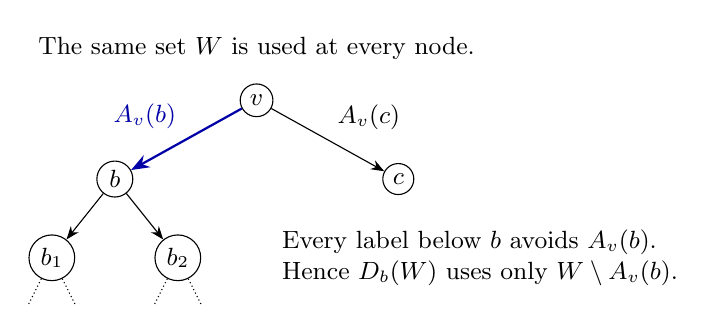
\begin{tikzpicture}[x=1cm,y=1cm,>=Stealth,
  vertex/.style={circle,draw,fill=white,inner sep=2pt},
  every node/.style={font=\small}]
\node[vertex] (v) at (0,0) {$v$};
\node[vertex] (b) at (-1.8,-1.0) {$b$};
\node[vertex] (c) at (1.8,-1.0) {$c$};
\node[vertex] (b1) at (-2.6,-2.0) {$b_1$};
\node[vertex] (b2) at (-1.0,-2.0) {$b_2$};
\draw[->,thick,blue!65!black] (v)--node[above left] {$A_v(b)$} (b);
\draw[->] (v)--node[above right] {$A_v(c)$} (c);
\draw[->] (b)--(b1);
\draw[->] (b)--(b2);
\draw[densely dotted] (b1)--(-2.9,-2.6);
\draw[densely dotted] (b1)--(-2.3,-2.6);
\draw[densely dotted] (b2)--(-1.3,-2.6);
\draw[densely dotted] (b2)--(-0.7,-2.6);
\node[align=left,anchor=west] at (0.2,-2.0)
  {Every label below $b$ avoids $A_v(b)$.\\
   Hence $D_b(W)$ uses only $W\setminus A_v(b)$.};
\node[anchor=south] at (0,0.4) {The same set $W$ is used at every node.};
\end{tikzpicture}
\caption{Every arc below $b$ lies on a path through the arc into $b$,
so the potential $D_b$ is a function of coordinates outside
$A_v(b)$. The diagram is schematic; labels on different branches (for
instance $A_v(c)$ and labels below $b$) may overlap.}
\label{fig:outside}
\end{figure}

\step{5}{expected potential: one level}
Now let $W\sim\mu_\rho$. Let $v$ have outgoing level $j$. By Step~4 we
may apply (M2) with $f=D_b$ for each child $b$; with (M1) and
$\epsilon_j^{-1}=\ee^{m_j}$, taking expectations in
\eqref{eq:pruning-recurrence} gives
\begin{equation}\label{eq:expected-potential}
 \EE D_v(W)
 \le\ee^{m_j}\Bigl(\ee^{-9m_j}
    +\ee^{11m_j}\sum_{b}\nu_v(b)\,\EE D_b(W)\Bigr)
 =\ee^{-8m_j}
    +\ee^{12m_j}\sum_{b\in\ch(v)}\nu_v(b)\,\EE D_b(W).
\end{equation}
This is the step that controls the dependence caused by reusing $W$:
the transition at $v$ and the potential $D_b$ both depend on $W$, and
\eqref{eq:distortion} decouples them at the cost $\ee^{11m_j}$.

\step{6}{solving the recursion}
For $1\le j\le k$ let $\beta_j$ be the maximum of $\EE D_v(W)$ over
nodes $v$ with outgoing level $j$, and put $\beta_{k+1}=0$ (leaves).
The children of a node with outgoing level $j$ have outgoing level
$j+1$ (or are leaves if $j=k$), and the weights $\nu_v(b)$ sum to $1$,
so \eqref{eq:expected-potential} gives
$\beta_j\le\ee^{-8m_j}+\ee^{12m_j}\beta_{j+1}$. We claim that for
$1\le j\le k+1$
\begin{equation}\label{eq:beta}
 \beta_j\le
 \sum_{i=j}^k
 \exp\Bigl(12\sum_{g=j}^{i-1}m_g-8m_i\Bigr),
\end{equation}
by downward induction on $j$. For $j=k+1$ both sides are $0$. If
\eqref{eq:beta} holds for $j+1$, then
\[
 \beta_j\le\ee^{-8m_j}
 +\ee^{12m_j}\sum_{i=j+1}^k
 \exp\Bigl(12\sum_{g=j+1}^{i-1}m_g-8m_i\Bigr)
 =\ee^{-8m_j}
 +\sum_{i=j+1}^k
 \exp\Bigl(12\sum_{g=j}^{i-1}m_g-8m_i\Bigr),
\]
and $\ee^{-8m_j}$ is the term $i=j$ of \eqref{eq:beta} (its inner sum
is empty). Now take $j=1$. Since
$m_g\le16^{-(i-g)}m_i$, we have
$\sum_{g<i}m_g\le m_i\sum_{x\ge1}16^{-x}=m_i/15$, so each exponent in
\eqref{eq:beta} is at most
$(\frac{12}{15}-8)m_i\le-7m_i$. The $m_i$ are distinct positive
integers because $m_{i+1}\ge16m_i>m_i$. Let $o$ be the root. By Step~3
and Markov's inequality,
\[
 \PP(o\text{ is bad})\le\PP(D_o(W)>1)\le\EE D_o(W)\le\beta_1
 \le\sum_{i=1}^k\ee^{-7m_i}
 \le\sum_{x\ge1}\ee^{-7x}=\frac1{\ee^7-1}<\frac14 .
\]
So the attempt succeeds with probability at least $\frac34$.

\step{7}{the reduced tree}
Fix $W$ for which the root is good. Start from the root. At any good
node $v$ with outgoing level $j$ put
\[
 \gamma_v(W)=\sum_{b\ \mathrm{good}}t_{vb}(W)\ge1-\epsilon_j>0 .
\]
Retain each good child $b$ with $t_{vb}(W)>0$, give it weight
$t_{vb}(W)/\gamma_v(W)$, replace its incoming label by
\[
 T_b=A_v(b)\setminus W,
\]
and continue recursively into $b$. Call the result $\TT'$. Every
retained node is good. The quantities $t_{vb}(W)$ define the
construction deterministically; sources and targets are auxiliary
random variables used only to define and analyse these numbers.

\step{8}{verification of the conclusions}
\emph{Probability tree with $k$ levels.} The new weights at a retained
node are positive and sum to $1$. Since $\gamma_v>0$, every retained
non-leaf node has at least one retained child, so all leaves of $\TT'$
are leaves of $\TT$, at depth $k$.

\emph{Disjoint.} Paths of $\TT'$ are paths of $\TT$ and
$T_b\subseteq A_v(b)$.

\emph{Capacity.} A retained arc has $t_{vb}(W)>0$, so
$|T_b|\le\lfloor m_j/2\rfloor$ by (M4).

\emph{Recovery \eqref{eq:recovery}.} A path $Q$ of $\TT'$ is, as a
sequence of nodes, a path $P$ of $\TT$, and
$A_v(b)\subseteq W\cup T_b$ on each of its arcs. Taking unions gives
$\UU(P)\subseteq W\cup\UU(Q)$.

\emph{Spread.} Let $v$ be a retained node with outgoing level $j$ and
$\varnothing\ne J\subseteq X$. Under the new child law the probability
that the label contains $J$ is
\[
 \frac1{\gamma_v(W)}
 \sum_{\substack{b\ \mathrm{good}\\ J\subseteq A_v(b)\setminus W}}
 t_{vb}(W).
\]
Consider the transition at $v$ at this fixed $W$. Since
$t_{vb}(W)\le\PP(\tgt=b\mid W)$, and on $\{\tgt=b\}$ the fragment is
$T=A_v(b)\setminus W$, the sum is at most $\PP(J\subseteq T\mid W)$. By
(P1), $T\subseteq A_v(\src)$, and at fixed $W$ the source has law
$\nu_v$ (see ``Two regimes''). Therefore
\[
 \PP(J\subseteq T\mid W)\le\PP_{c\sim\nu_v}(J\subseteq A_v(c))
 \le\alpha_j^{|J|},
\]
since level $j$ of $\TT$ is $\alpha_j$-spread. Dividing by
$\gamma_v(W)\ge1-\epsilon_j$ and using $|J|\ge1$,
\[
 \frac{\alpha_j^{|J|}}{1-\epsilon_j}
 \le\left(\frac{\alpha_j}{1-\epsilon_j}\right)^{|J|},
 \qquad \epsilon_j=\ee^{-m_j}.
\]
This proves (i) and (ii).
\end{proof}

\subsection{Iteration}

\begin{proof}[Proof of Theorem~\ref{thm:tree}]
\emph{Plan.} Apply Lemma~\ref{lem:reduction} repeatedly with fresh
independent sets. Each success halves all capacities. After
$s=\lfloor\log_2\ell_k\rfloor+1$ successes all labels are empty, and
the union of the successful sets contains a path union of $\TT$. With
probability at least $\frac23$ this takes at most $4s$ attempts, and
the union of $4s$ sets of density $\rho$ has density at most $r$.

\step{0}{parameters}
If $r=1$ then $W=X$ almost surely and the conclusion is immediate.
Suppose $r<1$, so that $r=16\ee^{50}\sigma(1+\log_2\ell_k)$, and set
\[
 a=4\sigma,\qquad \rho=\ee^{50}a=4\ee^{50}\sigma,
 \qquad s=\lfloor\log_2\ell_k\rfloor+1.
\]
Since $1+\log_2\ell_k\ge1$, we get
$\rho\le r/4<1$, so $0<\rho<1$.

\step{1}{arithmetic of capacities and spread}
For integers $\tau\ge0$ and $1\le i\le k$ define
\begin{equation}\label{eq:capacities}
 m_i(\tau)=\left\lfloor\frac{\ell_i}{2^\tau}\right\rfloor,
\end{equation}
which is nonincreasing in $\tau$. For the pairs $(i,\tau)$ with
$\tau=0$ or $m_i(\tau-1)\ge1$ define
\begin{equation}\label{eq:spread-iteration}
 \alpha_i(\tau)=\sigma
 \prod_{u=0}^{\tau-1}
 \left(1-\ee^{-m_i(u)}\right)^{-1}.
\end{equation}
For such a pair, $m_i(u)\ge m_i(\tau-1)\ge1$ for all $0\le u\le\tau-1$,
so every factor is finite and positive. These pairs include every
$(i,\tau)$ with $m_i(\tau)\ge1$, that is, every level still present
after $\tau$ successes; $\alpha_i(\tau)$ is not needed for other pairs,
except for a level in the round in which its capacity drops to $0$.
\begin{enumerate}[label=(A\arabic*),leftmargin=2.8em,itemsep=2pt]
 \item $\lfloor m_i(\tau)/2\rfloor=m_i(\tau+1)$, because
 $\lfloor\lfloor x\rfloor/2\rfloor=\lfloor x/2\rfloor$ for real
 $x\ge0$ (an integer $z$ satisfies $z\le x/2$ iff $2z\le x$ iff
 $2z\le\lfloor x\rfloor$).
 \item $m_i(\tau)$ is nondecreasing in $i$, so for each $\tau$ the
 levels with $m_i(\tau)=0$ form an initial segment
 $i=1,\ldots,k_0$. Moreover $m_{i+1}(\tau)\ge16m_i(\tau)$, because
 $16m_i(\tau)$ is an integer not exceeding
 $16\ell_i/2^\tau\le\ell_{i+1}/2^\tau$.
 \item $m_k(\tau)\ge1$ iff $2^\tau\le\ell_k$ iff $\tau\le s-1$. In
 particular $m_i(s)=0$ for all $i$.
 \item $0<\alpha_i(\tau)\le4\sigma=a$ whenever $\alpha_i(\tau)$ is
 defined. The integers $m_i(u)$, $0\le u\le\tau-1$, are at least $1$
 (as just noted) and strictly decreasing in $u$: by (A1),
 $m_i(u+1)=\lfloor m_i(u)/2\rfloor<m_i(u)$ because $m_i(u)\ge1$. Hence
 they are distinct positive integers, and the product in
 \eqref{eq:spread-iteration} is at most
 $\prod_{x\ge1}(1-\ee^{-x})^{-1}$. Using
 $-\log(1-y)\le y/(1-y)$ for $0\le y<1$ and $\ee^{-x}\le\ee^{-1}$,
 \begin{equation}\label{eq:product}
 \sum_{x=1}^{\infty}-\log(1-\ee^{-x})
 \le \frac{1}{1-\ee^{-1}}\sum_{x=1}^{\infty}\ee^{-x}
 =\frac{\ee^{-1}}{(1-\ee^{-1})^2}<0.93<\log 4,
 \end{equation}
 and exponentiating gives a product less than $4$.
\end{enumerate}

\step{2}{the procedure}
Let $W_1,W_2,\ldots$ be independent sets of law $\mu_\rho$. Maintain a
\emph{current tree}, initially $\TT$. At attempt $\lambda=1,2,\ldots$,
if the current tree has at least one level, run the procedure of
Lemma~\ref{lem:reduction} on it with the set $W_\lambda$.
\begin{itemize}[leftmargin=1.6em,itemsep=2pt]
 \item On failure, leave the current tree unchanged.
 \item On success, let $\TT'$ be the returned tree, with $k'$ levels,
 and \emph{trim} it: let $k_0\le k'$ be the number of its levels whose
 new capacity is $0$ (an initial segment, by (A2)); choose by a fixed
 rule a node $o'$ of $\TT'$ at depth $k_0$; the new current tree is the
 subtree of $\TT'$ rooted at $o'$, with its labels and child laws. Such
 a node exists because every root-to-leaf path of $\TT'$ has a node at
 each depth $0,\ldots,k'$; if $k_0=k'$ it is a leaf and the new current
 tree is a single node.
\end{itemize}
Stop when the current tree has no levels (a single node).

\emph{Trimming is harmless.} The subtree rooted at $o'$ is a probability
tree with $k'-k_0$ levels (the leaves of $\TT'$ have depth $k'$). It is
disjoint, since each of its paths is part of a path of $\TT'$. Its
labels and child laws are those of $\TT'$, so every capacity and spread
bound of $\TT'$ at a retained level still holds. If $Q'$ is a path of
the subtree, then the path of $\TT'$ from its root to $o'$ followed by
$Q'$ is a path $Q$ of $\TT'$; its first $k_0$ labels are empty, so
$\UU(Q)=\UU(Q')$.

\step{3}{invariants}
Let $\TT_\tau$ be the current tree after $\tau$ successes and
$\overline W_\tau$ the union of the $\tau$ sets $W_\lambda$ of the
successful attempts so far ($\overline W_0=\varnothing$). We claim, for
every $\tau$ reached:
\begin{enumerate}[label=(I\arabic*),leftmargin=2.6em,itemsep=2pt]
 \item $\TT_\tau$ is a disjoint probability tree whose levels correspond,
 in order, to the original levels $i$ with $m_i(\tau)\ge1$, and the level
 corresponding to $i$ has capacity $m_i(\tau)$;
 \item that level is $\alpha_i(\tau)$-spread;
 \item for every path $Q$ of $\TT_\tau$ there is a path $P$ of $\TT$
 with $\UU(P)\subseteq\overline W_\tau\cup\UU(Q)$.
\end{enumerate}
For $\tau=0$ these are the hypotheses of the theorem. Assume them for
$\tau$, with $\TT_\tau$ having at least one level, and let $W$ be the
set of the next successful attempt. By (I1), (I2), (A2), (A4) and
Step~0, $\TT_\tau$ satisfies the hypotheses of
Lemma~\ref{lem:reduction} with capacities $m_i(\tau)\ge1$, spread
parameters $\alpha_i(\tau)\le a$ and $\rho=\ee^{50}a<1$. Its conclusion
(i) and (A1) give capacities $m_i(\tau+1)$ and spread
$\alpha_i(\tau)/(1-\ee^{-m_i(\tau)})=\alpha_i(\tau+1)$ for $\TT'$.
Trimming removes exactly the levels with $m_i(\tau+1)=0$ and preserves
the rest, giving (I1) and (I2) for $\tau+1$. For (I3): given a path
$Q'$ of $\TT_{\tau+1}$, trimming gives a path $Q$ of $\TT'$ with
$\UU(Q)=\UU(Q')$; conclusion (ii) gives a path $P'$ of $\TT_\tau$ with
$\UU(P')\subseteq W\cup\UU(Q)$; and (I3) for $\tau$ gives a path $P$ of
$\TT$ with
\[
 \UU(P)\subseteq\overline W_\tau\cup\UU(P')
 \subseteq\overline W_\tau\cup W\cup\UU(Q')
 =\overline W_{\tau+1}\cup\UU(Q').
\]
Only successful draws enter $\overline W_\tau$: a failed attempt changes
nothing.

\step{4}{completion}
By (I1) and (A3), $\TT_\tau$ has at least one level for $\tau\le s-1$
and none for $\tau=s$. So the procedure stops exactly at the $s$-th
success. The unique path of the single-node tree $\TT_s$ has empty
union, so (I3) gives a path $P$ of $\TT$ with
$\UU(P)\subseteq\overline W_s$.

\step{5}{number of attempts}
\emph{Conditional success probability.} Fix $\lambda\ge1$ and sets
$w_1,\ldots,w_{\lambda-1}\subseteq X$ such that, when
$W_1=w_1,\ldots,W_{\lambda-1}=w_{\lambda-1}$, the procedure has not
stopped before attempt $\lambda$. Then the current tree before attempt
$\lambda$ is one fixed tree, a function of
$w_1,\ldots,w_{\lambda-1}$ (Lemma~\ref{lem:reduction} is deterministic
and trimming uses a fixed rule); by Step~3 it satisfies the hypotheses
of Lemma~\ref{lem:reduction}; and $W_\lambda$ is independent of
$W_1,\ldots,W_{\lambda-1}$ with law $\mu_\rho$. Hence
\begin{equation}\label{eq:cond-fail}
 \PP\bigl(\text{attempt }\lambda\text{ fails}\bigm|
 W_1=w_1,\ldots,W_{\lambda-1}=w_{\lambda-1}\bigr)\le\tfrac14 .
\end{equation}
Consequently, if $E$ is an event determined by
$W_1,\ldots,W_{\lambda-1}$ on which the procedure has not stopped before
attempt $\lambda$, then
\begin{equation}\label{eq:cond-event}
 \PP\bigl(E\cap\{\text{attempt }\lambda\text{ fails}\}\bigr)
 \le\tfrac14\,\PP(E):
\end{equation}
multiply \eqref{eq:cond-fail} by
$\PP(W_1=w_1,\ldots,W_{\lambda-1}=w_{\lambda-1})$ and sum over the
finitely many tuples that make up $E$.

\emph{Waiting times.} For $0\le i\le s$ let $\Lambda_i$ be the index of
the attempt at which the $i$-th success occurs ($\Lambda_0=0$), and
$\Delta_i=\Lambda_i-\Lambda_{i-1}$ for $1\le i\le s$. We show by
induction on $i$ that $\Lambda_{i-1}<\infty$ almost surely and
$\PP(\Delta_i>x)\le4^{-x}$ for every integer $x\ge0$. Assume
$\Lambda_{i-1}<\infty$ almost surely (true for $i=1$). For integers
$\lambda,x\ge0$ let
\[
 E_{\lambda,x}=\{\Lambda_{i-1}=\lambda\text{ and attempts }
 \lambda+1,\ldots,\lambda+x\text{ all fail}\}.
\]
This event is determined by $W_1,\ldots,W_{\lambda+x}$, and on it only
$i-1\le s-1$ successes occur among the first $\lambda+x$ attempts, so
by Step~4 the procedure has not stopped before attempt $\lambda+x+1$.
Since
$E_{\lambda,x+1}=E_{\lambda,x}\cap\{\text{attempt }\lambda+x+1
\text{ fails}\}$, \eqref{eq:cond-event} gives
$\PP(E_{\lambda,x+1})\le\frac14\PP(E_{\lambda,x})$. Up to a null set,
$\{\Delta_i>x\}$ is the disjoint union of the events $E_{\lambda,x}$
over $\lambda\ge0$. Summing over $\lambda$,
\[
 \PP(\Delta_i>x+1)\le\tfrac14\,\PP(\Delta_i>x),
 \qquad\text{hence}\qquad\PP(\Delta_i>x)\le4^{-x}.
\]
In particular $\Delta_i<\infty$ and so $\Lambda_i<\infty$ almost
surely, which completes the induction.

\emph{Markov bound.} Therefore
\[
 \EE\Delta_i=\sum_{x\ge0}\PP(\Delta_i>x)\le\sum_{x\ge0}4^{-x}=\tfrac43,
 \qquad
 \EE\Lambda_s=\sum_{i=1}^s\EE\Delta_i\le\tfrac43s .
\]
By Markov's inequality
$\PP(\Lambda_s\ge4s+1)\le\frac{4s/3}{4s+1}<\frac13$, so
$\PP(\Lambda_s\le4s)\ge\frac23$.

\step{6}{one sample of density $r$}
Let $W_*=W_1\cup\cdots\cup W_{4s}$ (all $4s$ sets, including any that
the procedure does not use). On the event $\{\Lambda_s\le4s\}$
all successful draws are among $W_1,\ldots,W_{4s}$, so
$\overline W_s\subseteq W_*$ and, by Step~4, $W_*$ contains $\UU(P)$
for some path $P$ of $\TT$. This has probability at least $\frac23$.
Each element of $X$ lies in $W_*$ independently with probability
\[
 r_*=1-(1-\rho)^{4s}
 \le4s\rho
 =16\ee^{50}\sigma s
 \le16\ee^{50}\sigma(1+\log_2\ell_k)=r,
\]
using Bernoulli's inequality and
$s\le1+\log_2\ell_k$. So $W_*\sim\mu_{r_*}$ with $r_*\le r$. The event
``$W$ contains $\UU(P)$ for some path $P$'' is increasing in $W$, and
$\mu_{r_*}$ and $\mu_r$ can be coupled so that the first set is
contained in the second (take independent uniform variables $U_e$,
$e\in X$, and the sets $\{e:U_e\le r_*\}\subseteq\{e:U_e\le r\}$). Hence
the probability under $\mu_r$ is also at least $\frac23$.
\end{proof}

\section{Application to graph containment}\label{sec:graphs}

It remains to construct the tree required by Theorem~\ref{thm:tree}.
The construction is the normalized-containment maximization and
conditional-extension argument of
Tran~\cite[Section~3, Lemma~3.1]{Tran26}, with constants suited to the
factor-$16$ separation of capacities; it is proved in full here.

\paragraph{Standing notation.}
Fix $n\ge2$ and $H$ as in Theorem~\ref{thm:main}, and put
\[
 \qs=\pE(n,H),\qquad\sigma=128\qs,\qquad X=\tbinom{[n]}2 .
\]
Here $\qs$ is a number, always defined from the original graph $H$ with
all its subgraphs. By facts (a) and (b) of
Section~\ref{sec:introduction}, $\qs>0$ and the constraints defining
$\pE$ hold at $p=\qs$.

\paragraph{Edge-set convention.}
A graph without isolated vertices is determined by its edge set, and we
identify the two. So $E(H)$ denotes both the edge set of $H$ and the
graph obtained from $H$ by deleting its isolated vertices, and an
\emph{edge set} $F\subseteq E(H)$ is regarded as the graph formed by
the edges of $F$ and their endpoints. That graph has no isolated
vertices and is a subgraph of $H$ in the sense of
Section~\ref{sec:introduction}, so it is one of the graphs constrained
in the definition of $\pE(n,H)$. These are the only constraints of
$\pE$ that the proof uses; the constraints coming from subgraphs with
isolated vertices are never needed. A subgraph of $K_n$ isomorphic to
such an $F$ again has no isolated vertices and is determined by its
edge set, so a \emph{copy} of $F$ in $K_n$ may be regarded as a subset
of $X$, and counting copies as subgraphs or as edge sets gives the same
number. For edge sets $F$ and $I$ let
\[
 M(F)=N(K_n,F),\qquad M(I,F)=N(I,F),
\]
the numbers of copies of $F$ in $K_n$ and in $I$; equivalently,
$M(I,F)$ is the number of subsets of $I$ that are isomorphic to $F$ as
graphs. These count copies, not vertex embeddings. For the empty edge
set, $M(\varnothing)=M(I,\varnothing)=1$. We use four facts.
\begin{enumerate}[label=(F\arabic*),leftmargin=2.6em,itemsep=3pt]
 \item \emph{A graph on $[n]$ contains a copy of $H$ if and only if its
 edge set contains a copy of $E(H)$.} For ``if'': the copy of $E(H)$
 uses $v(H)$ minus the number of isolated vertices of $H$ many
 vertices; since $n\ge v(H)$, enough further vertices of $[n]$ remain
 to serve as the isolated vertices, and copies need not be induced.
 ``Only if'' is clear.
 \item \emph{For every nonempty $F\subseteq E(H)$,
 $M(F)\qs^{|F|}\ge\frac12$.} By the convention above the graph of $F$
 is a subgraph of $H$, so its constraint holds at $\qs$:
 $\EE N(G(n,\qs),F)\ge\frac12$. By \eqref{eq:expect}, with
 $N(K_n,F)=M(F)$ and $e(F)=|F|$, the left side is $M(F)\qs^{|F|}$.
 \item \emph{If $F\subseteq F'\subseteq E(H)$, every copy $S_0$ of $F$
 in $K_n$ is contained in a copy of $F'$ in $K_n$.} Take an isomorphism
 from $F$ to $S_0$, a bijection $\phi$ between their vertex sets. Since
 $F'$ has at most $v(H)\le n$ vertices, $\phi$ extends to an injection
 of the vertex set of $F'$ into $[n]$; the image of $F'$ is a copy of
 $F'$ containing $S_0$. In particular (take $F=\varnothing$) copies of
 $F'$ exist.
 \item \emph{Copy ratio.} For an edge set $I\subseteq E(H)$ let $\GG_I$
 be a uniformly random copy of $I$ in $K_n$. If $F\subseteq I$ and
 $F_0$ is any fixed copy of $F$ in $K_n$, then
 \begin{equation}\label{eq:copy-ratio}
  \PP(F_0\subseteq\GG_I)=\frac{M(I,F)}{M(F)}.
 \end{equation}
\end{enumerate}

\begin{proof}[Proof of (F4)]
A permutation $\pi$ of $[n]$ acts on $X$ and maps copies of an edge set
to copies of the same edge set, so $\pi(\GG_I)$ is again uniform on the
copies of $I$. Any two copies $F_0,F_0'$ of $F$ satisfy
$F_0'=\pi(F_0)$ for some $\pi$ (extend an isomorphism between them to a
permutation of $[n]$). Hence
$\PP(F_0'\subseteq\GG_I)=\PP(F_0\subseteq\pi^{-1}(\GG_I))
=\PP(F_0\subseteq\GG_I)$: the probability is the same number $\theta$
for all copies. Summing over the $M(F)$ copies of $F$ counts the copies
of $F$ contained in $\GG_I$; there are exactly $M(I,F)$ of them because
$\GG_I$ is isomorphic to $I$. So $M(F)\theta=M(I,F)$.
\end{proof}

\begin{lemma}[Graph hierarchy]\label{lem:hierarchy}
There is a disjoint probability tree on
$X=\binom{[n]}2$ whose path unions are copies of $H$ with its isolated
vertices removed, such that every level is $\sigma$-spread and its label
sizes $\ell_1,\ldots,\ell_k$ satisfy
\[
 1\le\ell_1,\qquad \ell_{i+1}\ge16\ell_i,
 \qquad \ell_k\le e(H).
\]
\end{lemma}

Here $k\ge1$, and every label of level $i$ has exactly $\ell_i$
elements, so level $i$ has capacity $\ell_i$. \emph{Use:} this is the
input to Theorem~\ref{thm:tree} in the proof of
Theorem~\ref{thm:main}.

\begin{proof}
\emph{Plan.} For an edge set $I$, choose $S\subseteq I$ maximizing a
normalized containment probability. The constraints (F2) force
$|S|<|I|/17$ (Step~1). Iterating from $I=E(H)$ gives a chain
(Step~2), the tree records all ways to extend copies along the chain
(Step~3), and maximality gives spread (Step~5).

\step{1}{the maximizer is small}
For a nonempty edge set $I\subseteq E(H)$ and $S\subseteq I$ let
\begin{equation}\label{eq:maximizer}
 R_\sigma(I,S)=\sigma^{-|S|}\,\PP(S_0\subseteq\GG_I)
 =\sigma^{-|S|}\,\frac{M(I,S)}{M(S)},
\end{equation}
where $S_0$ is any fixed copy of $S$; by (F4) this depends only on the
isomorphism type of $S$. Choose $S\subseteq I$ maximizing
$R_\sigma(I,S)$, breaking ties by a fixed rule. Since
$R_\sigma(I,\varnothing)=1$, the maximum is at least $1$. We claim that
$|S|<|I|/17$. This is clear if $S=\varnothing$. Otherwise write
$h_I=|I|$ and $\kappa=|S|\ge1$. By (F2), $1/M(S)\le2\qs^\kappa$, and
$M(I,S)\le\binom{h_I}{\kappa}$ since copies of $S$ in $I$ are
$\kappa$-element subsets of $I$. Hence
\[
 R_\sigma(I,S)\le2\binom{h_I}{\kappa}(\qs/\sigma)^\kappa
           =2\binom{h_I}{\kappa}128^{-\kappa}.
\]
If $\kappa\ge h_I/17$, the bound
$\binom{h_I}{\kappa}\le(\ee h_I/\kappa)^\kappa\le(17\ee)^\kappa$ gives
\[
 R_\sigma(I,S)\le2(17\ee/128)^\kappa\le2\cdot\frac{17\ee}{128}<0.73<1,
\]
contradicting $R_\sigma(I,S)\ge1$.

\step{2}{the chain}
Start with $I=E(H)$ and repeatedly replace $I$ by its chosen maximizer
until the empty set is reached; sizes strictly decrease, so this
terminates. Writing the sequence in reverse order,
\[
 \varnothing=H_0\subset H_1\subset\cdots\subset H_k=E(H),
 \qquad |H_{i-1}|<|H_i|/17,
\]
where $H_{i-1}$ maximizes $R_\sigma(H_i,\cdot)$ over subsets of $H_i$,
and $k\ge1$ because $E(H)\ne\varnothing$. Put
\[
 \ell_i=|H_i|-|H_{i-1}|>0 .
\]
Then $\ell_1\ge1$, $\ell_k\le|E(H)|=e(H)$, and
$\ell_{i+1}>17|H_i|-|H_i|=16|H_i|\ge16\ell_i$.

\step{3}{the tree}
The root is the empty edge set (the unique copy of $H_0$). A node at
depth $i-1$ is a history of nested copies ending in a copy $S_0$ of
$H_{i-1}$; distinct histories are distinct nodes. Its children are all
copies $I_0$ of $H_i$ in $K_n$ with $S_0\subseteq I_0$, with the uniform
distribution, and the arc to $I_0$ is labelled $I_0\setminus S_0$. By
(F3) every node at depth $i-1<k$ has at least one child, so all leaves
have depth $k$.

\step{4}{disjointness, path unions, label sizes}
Along a path the copies are nested,
$\varnothing=S^0\subseteq S^1\subseteq\cdots\subseteq S^k$, and the
labels are the differences $S^i\setminus S^{i-1}$. They are pairwise
disjoint, their union is $S^k$, a copy of $H_k=E(H)$, and
$|S^i\setminus S^{i-1}|=|H_i|-|H_{i-1}|=\ell_i$.

\step{5}{every level is $\sigma$-spread}
Fix a node at depth $i-1$ with current copy $S_0$ of $H_{i-1}$, and let
$A$ be the random label of the arc to a random child. The child is
uniform among the copies of $H_i$ containing $S_0$, that is, it has the
law of $\GG_{H_i}$ conditioned on $S_0\subseteq\GG_{H_i}$, an event of
positive probability by (F3). Let $\varnothing\ne J\subseteq X$. If
$J\cap S_0\ne\varnothing$, then $\PP(J\subseteq A)=0$. Otherwise
\begin{equation}\label{eq:conditional-ratio}
 \PP(J\subseteq A)=
 \frac{\PP(S_0\cup J\subseteq\GG_{H_i})}
      {\PP(S_0\subseteq\GG_{H_i})}.
\end{equation}
If the numerator is zero the bound $\PP(J\subseteq A)\le\sigma^{|J|}$
is trivial. If it is positive, $S_0\cup J$ lies in some copy of $H_i$;
pulling back along the isomorphism from $H_i$ to that copy shows that
$S_0\cup J$ is a copy of some edge set $U\subseteq H_i$ with
$|U|=|S_0|+|J|$. By \eqref{eq:maximizer} and (F4),
$R_\sigma(H_i,U)=\sigma^{-|S_0|-|J|}\PP(S_0\cup J\subseteq\GG_{H_i})$
and
$R_\sigma(H_i,H_{i-1})=\sigma^{-|S_0|}\PP(S_0\subseteq\GG_{H_i})$.
Maximality of $H_{i-1}$ among subsets of $H_i$ gives
$R_\sigma(H_i,U)\le R_\sigma(H_i,H_{i-1})$, that is,
\[
 \sigma^{-(|S_0|+|J|)}\PP(S_0\cup J\subseteq\GG_{H_i})
 \le \sigma^{-|S_0|}\PP(S_0\subseteq\GG_{H_i}).
\]
With \eqref{eq:conditional-ratio} this is
$\PP(J\subseteq A)\le\sigma^{|J|}$.
\end{proof}

\begin{proof}[Proof of Theorem~\ref{thm:main}]
Apply Theorem~\ref{thm:tree} to the tree of Lemma~\ref{lem:hierarchy},
with $\sigma=128\qs>0$ and capacities $\ell_1,\ldots,\ell_k$. It shows
that a random subset of $X$ of density
$r'=\min\{1,16\ee^{50}\cdot128\qs(1+\log_2\ell_k)\}$ contains a path
union, that is, a copy of $E(H)$, with probability at least $\frac23$.
Since $16\cdot128=2048$ and $\ell_k\le h=e(H)$,
\[
 r'\le r:=\min\{1,\;2048\ee^{50}\qs(1+\log_2 h)\},
\]
and by the monotone coupling of Step~6 in the proof of
Theorem~\ref{thm:tree} the same holds at density $r$. The edge set of
$G(n,r)$ has law $\mu_r$, so by (F1),
$\PP(N(G(n,r),H)>0)\ge\frac23\ge\frac12$, and $\pc(n,H)\le r$ by the
definition of $\pc$. As $\qs=\pE(n,H)$, this proves
\eqref{eq:stronger}. Finally,
$h\le\binom n2\le n^2$ and $\log_2n\ge1$ for $n\ge2$ give
$1+\log_2 h\le1+2\log_2n\le3\log_2 n$, and $3\cdot2048=6144$, which is
the stated constant $6144\ee^{50}$.
\end{proof}

\section{Verification checklist}

No step of this rewrite carries an ``Unverified step'' box: each step
of the source was rechecked while writing and none raised a doubt. That
is a report, not evidence; the list below says where a sceptical reader
should look first.

\begin{enumerate}[leftmargin=2em,itemsep=3pt]
 \item \textbf{The one-pair computation \eqref{eq:onepair}}
 (Lemma~\ref{lem:local}, Step~3). Check the cancellation
 $\rho^{-|A_b|}\rho^{|A_b\setminus A_c|}=\rho^{-|A_c\cap A_b|}$ and that
 independence needs $f$ to ignore $W\cap A_b$. Both conclusions of
 Lemma~\ref{lem:local} follow from it, \eqref{eq:grouping} and
 (P4).
 \item \textbf{$D_b$ depends only on $W\setminus A_v(b)$}
 (Lemma~\ref{lem:reduction}, Step~4). This is the only use of
 disjointness along paths in the probability estimate, and it is what
 allows \eqref{eq:distortion} to be applied with $f=D_b$ in Step~5
 although the same $W$ is used at all nodes.
 \item \textbf{The exponents in the potential recursion}
 (Lemma~\ref{lem:reduction}, Steps~5--6):
 $\ee^{m_j}\cdot\ee^{-9m_j}$ and $\ee^{m_j}\cdot\ee^{11m_j}$ in
 \eqref{eq:expected-potential}, the induction for \eqref{eq:beta}, and
 $12\cdot\frac1{15}-8\le-7$ from the factor-$16$ growth, giving failure
 probability below $\frac14$.
 \item \textbf{Spread of the reduced tree}
 (Lemma~\ref{lem:reduction}, Step~8). It uses that at fixed $W$ the
 source still has law $\nu_v$, that $T\subseteq A_v(\src)$ by (P1), and
 that the normalization is $\gamma_v\ge1-\ee^{-m_j}$.
 \item \textbf{Iteration bookkeeping} (Theorem~\ref{thm:tree},
 Steps~1--4): the product bound \eqref{eq:product}, which keeps the
 spread below $a=4\sigma$ in every round; the invariants (I1)--(I3),
 including why trimming zero-capacity levels preserves them; and
 completion after exactly $s$ successes.
 \item \textbf{From $s$ successes to density $r$}
 (Theorem~\ref{thm:tree}, Steps~5--6): the conditional bound
 \eqref{eq:cond-fail} given the whole history, the geometric tail of
 the waiting times, the Markov bound for $4s$ attempts, and
 $1-(1-\rho)^{4s}\le4s\rho\le r$.
 \item \textbf{The hierarchy} (Lemma~\ref{lem:hierarchy}): Step~1,
 where (F2) is the only use of the definition of $\pE$ and
 $2\cdot17\ee/128<1$ forces $|S|<|I|/17$; and Step~5, where maximality
 is applied to the isomorphism type $U$ of $S_0\cup J$ via (F4).
 \item \textbf{Constants} (proof of Theorem~\ref{thm:main}):
 $16\cdot128=2048$, $\ell_k\le h$, and $1+\log_2h\le3\log_2n$.
\end{enumerate}

\begin{thebibliography}{99}
\raggedright

\bibitem{ALWZ21}
R.~Alweiss, S.~Lovett, K.~Wu, and J.~Zhang,
\emph{Improved bounds for the sunflower lemma},
Annals of Mathematics (2) \textbf{194} (2021), no.~3, 795--815.
\href{https://doi.org/10.4007/annals.2021.194.3.5}{doi:10.4007/annals.2021.194.3.5}.

\bibitem{Bollobas81}
B.~Bollob\'as,
\emph{Threshold functions for small subgraphs},
Mathematical Proceedings of the Cambridge Philosophical Society
\textbf{90} (1981), no.~2, 197--206.
\href{https://doi.org/10.1017/S0305004100058655}{doi:10.1017/S0305004100058655}.

\bibitem{DKP25}
Q.~Dubroff, J.~Kahn, and J.~Park,
\emph{On the ``second'' Kahn--Kalai conjecture},
arXiv:2508.14269v1 (August 19, 2025).
\url{https://arxiv.org/abs/2508.14269v1}.

\bibitem{DKP25Cases}
Q.~Dubroff, J.~Kahn, and J.~Park,
\emph{On the ``second'' Kahn--Kalai conjecture: cliques, cycles, and trees},
arXiv:2510.02005v2 (October 23, 2025).
\url{https://arxiv.org/abs/2510.02005v2}.

\bibitem{ER60}
P.~Erd\H{o}s and A.~R\'enyi,
\emph{On the evolution of random graphs},
Publications of the Mathematical Institute of the Hungarian Academy of
Sciences \textbf{5} (1960), 17--61.
\url{https://static.renyi.hu/~p_erdos/1960-10.pdf}.

\bibitem{ER66}
P.~Erd\H{o}s and A.~R\'enyi,
\emph{On the existence of a factor of degree one of a connected random graph},
Acta Mathematica Academiae Scientiarum Hungaricae
\textbf{17} (1966), 359--368.
\url{https://users.renyi.hu/~p_erdos/1966-16.pdf}.

\bibitem{FKNP21}
K.~Frankston, J.~Kahn, B.~Narayanan, and J.~Park,
\emph{Thresholds versus fractional expectation-thresholds},
Annals of Mathematics (2) \textbf{194} (2021), no.~2, 475--495.
\href{https://doi.org/10.4007/annals.2021.194.2.2}{doi:10.4007/annals.2021.194.2.2}.

\bibitem{KK07}
J.~Kahn and G.~Kalai,
\emph{Thresholds and expectation thresholds},
Combinatorics, Probability and Computing
\textbf{16} (2007), no.~3, 495--502.
\href{https://doi.org/10.1017/S0963548307008474}{doi:10.1017/S0963548307008474}.

\bibitem{LSZ19}
S.~Lovett, N.~Solomon, and J.~Zhang,
\emph{From DNF compression to sunflower theorems via regularity},
34th Computational Complexity Conference, LIPIcs \textbf{137} (2019),
5:1--5:14.
\href{https://doi.org/10.4230/LIPIcs.CCC.2019.5}{doi:10.4230/LIPIcs.CCC.2019.5}.

\bibitem{MNSZ25}
E.~Mossel, J.~Niles-Weed, N.~Sun, and I.~Zadik,
\emph{A Bayesian proof of the spread lemma},
Random Structures \& Algorithms \textbf{66} (2025), no.~4, e70008.
\href{https://doi.org/10.1002/rsa.70008}{doi:10.1002/rsa.70008}.

\bibitem{MNSZ22}
E.~Mossel, J.~Niles-Weed, N.~Sun, and I.~Zadik,
\emph{On the second Kahn--Kalai conjecture},
arXiv:2209.03326v1 (September 7, 2022).
\url{https://arxiv.org/abs/2209.03326v1}.

\bibitem{OpenAIThresholdEquivalence2026}
OpenAI,
\emph{Integral and fractional expectation thresholds are equivalent},
OpenAI Math Release preprint
\href{https://github.com/openai/math/blob/main/preprints/Integral-and-fractional-expectation-thresholds-are-equivalent-September-23-2026/paper.pdf}{OAI:Integral-and-fractional-expectation-thresholds-are-equivalent-September-23-2026},
2026, Theorem~1.1, p.~2.

\bibitem{PP24}
J.~Park and H.~T.~Pham,
\emph{A proof of the Kahn--Kalai conjecture},
Journal of the American Mathematical Society
\textbf{37} (2024), no.~1, 235--243.
\href{https://doi.org/10.1090/jams/1028}{doi:10.1090/jams/1028}.

\bibitem{Riordan00}
O.~Riordan,
\emph{Spanning subgraphs of random graphs},
Combinatorics, Probability and Computing
\textbf{9} (2000), no.~2, 125--148.
\href{https://doi.org/10.1017/S0963548399004150}{doi:10.1017/S0963548399004150}.

\bibitem{Tal10}
M.~Talagrand,
\emph{Are many small sets explicitly small?},
Proceedings of the 42nd ACM Symposium on Theory of Computing (2010),
13--36.
\href{https://doi.org/10.1145/1806689.1806693}{doi:10.1145/1806689.1806693}.

\bibitem{Tran26}
T.~Tran,
\emph{Fractional expectation thresholds and the ``second'' Kahn--Kalai
conjecture},
arXiv:2609.20546v2 (September 24, 2026).
\url{https://arxiv.org/abs/2609.20546v2}.

\end{thebibliography}

\end{document}
